\documentclass{article}

\usepackage[UTF8]{ctex}
\usepackage{amsmath}
\usepackage{amsthm}
\usepackage{bm}
\usepackage{extarrows}
\usepackage{color}
\usepackage{mathrsfs}
\usepackage{amssymb}
\usepackage{booktabs}
\usepackage{algorithm} 
%\usepackage{algorithmic} 
\usepackage{algorithmicx}  
\usepackage{algpseudocode}  
\usepackage{listings}
\usepackage{multirow}
\usepackage{graphicx}
\usepackage{diagbox}
\usepackage{xcolor}
\usepackage[width=16cm]{geometry}


\geometry{a4paper,scale=0.8}
\newtheorem{theorem}{\hspace{2em}定理}
\newtheorem{lemma}{\hspace{2em}引理}
%\newtheorem{proof}{证明}
\floatname{algorithm}{算法}  
\renewcommand{\algorithmicrequire}{\textbf{输入:}}  
\renewcommand{\algorithmicensure}{\textbf{输出:}}  


\title{并行算法试题 答题卷}
\author{林宇健   2018202296}
\date{2019 年 2 月 10 日}

\begin{document}
\maketitle

%%%%%%%%%%%%%%%%%%%%%%%%%%%%%%%%%%%%%%%%%%%%%%%%%%%%%%%%%%%%%%%%%%%%%%%%%
%%%%%%%%%%%%%%%%%%%%%%%%%%%%%%%%%%%%%%%%%%%%%%%%%%%%%%%%%%%%%%%%%%%%%%%%%
\section{并行矩阵向量乘法}
\subsection{问题描述和算法分析}
编程计算$Ax$,其中$A$是$m\times n$的稠密矩阵,$x$是$n$维列向量,分别采用$1,4,8,16$台处理机计算。给出并行算法,及并行效率分析。

记$y=Ax$。为简便起见,取$A$是$n\times n$的方阵,$n = 2048$可以整除$1,4,8,16$,从而保证每个进程储存的向量块维度相同。对于不能整除$4,8,16$的$n$,可通过循环存储等方式为各个进程分配矩阵和向量的数据。在计算时编程随机生成了$matrix_{2048\times 2048}$和$vector_{2048 \times 1}$作为待计算的矩阵和向量(计算程序略去)。

我们采用一维行划分的方式并行计算矩阵向量乘法。假设矩阵$A$按逐行一维块划分为$p$个块($p$表示进程数),即$A = [A_{1}, A_{2}, \cdots, A_{p}]^{T},A_{k} = [A_{k,0},A_{k,1},\cdots,A_{k,p}]$。其中

\begin{center}	
	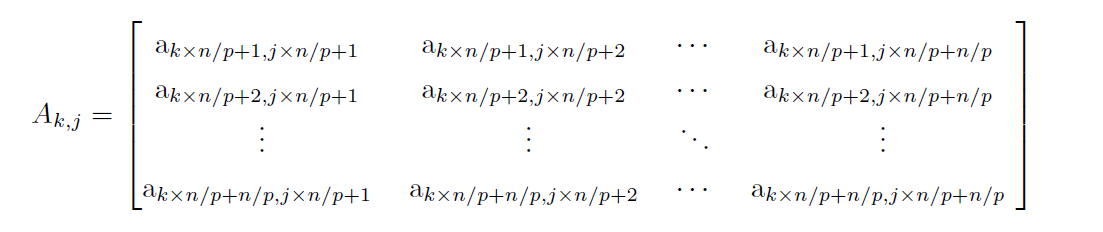
\includegraphics[width=1.0\linewidth]{pic01.png}
\end{center}

与之相对应,向量$x$和向量$y$也分为$p$个块,其第$k(0\leq k\leq p-1)$个块分别为

$$x_{k} = \left[\begin{matrix}
  x_{k\times n/p+1} & x_{k\times n/p+2} & \cdots & x_{k\times n/p+n/p}
\end{matrix}\right]^{T}\\$$

$$y_{k} = \left[\begin{matrix}
y_{k\times n/p+1} & y_{k\times n/p+2} & \cdots & y_{k\times n/p+n/p}
\end{matrix}\right]^{T}$$

假设$A_{k}$、$x_{k}$和$y_{k}$储存在进程$k$上,下图表示了对应的数据分布情况。

\begin{center}
	\renewcommand\tabcolsep{7pt}
	\begin{tabular}{cccc|c|c|ccc}
		\multicolumn{4}{c}{\bf{$A$}}& \multicolumn{1}{c}{ }& \multicolumn{1}{c}{\bf{$X$}}& &\\
		\cline{1-4} \cline{6-6}
		\multicolumn{1}{|c}{\bf{$A_{1,1}$}}& $A_{1,2}$& $\cdots$& $A_{1,p}$& & $x_{1}$& &$P_{1}$\\
		\cline{1-4}\cline{6-6}
		\cmidrule[0.25pt]{1-8}
		\cline{1-4}\cline{6-6}
		\multicolumn{1}{|c}{\bf{$A_{2,1}$}}& $A_{2,2}$& $\cdots$& $A_{2,p}$& & $x_{2}$& &$P_{2}$\\
		\cline{1-4}\cline{6-6}
		\cmidrule[0.25pt]{1-8}
		\cline{1-4}\cline{6-6}
		\multicolumn{1}{|c}{$\vdots$}& $\vdots$& $\ddots$& $\vdots$& & $\vdots$& &$\vdots$\\
		\cline{1-4}\cline{6-6}
		\cmidrule[0.25pt]{1-8}
		\cline{1-4}\cline{6-6}
		\multicolumn{1}{|c}{\bf{$A_{p,1}$}}& $A_{p,2}$& $\cdots$& $A_{p,p}$& & $x_{p}$& &$P_{p}$\\
		\cline{1-4}\cline{6-6}
	\end{tabular}
\end{center}

在特定的进程$k$上,需要计算的是对应的$y_{k}$,而$y_{k}$的计算公式如下

$$y_{k}=A_{k}x=\sum_{j=0}^{p-1}A_{k.j}x_{j}=\sum_{j=0}^{p-1}A_{k,(k+j)\% p}x_{(k+j)\% p}$$

其中$\%$表示取余运算。可以看出在计算$y_{k}$时给定的子矩阵$A$的行标号始终为$k$。在进行第$j$步的计算时,需要用到的$x$的子向量$x_{(k+j)\%p}$,所以可以通过每计算一次将$x$的块在同列进程中循环上移一个位置的方法实现,在计算到第$j$步的时候$x$的块正好循环上移了$j$次,即计算所用的$x$的子向量在当前进程上,从而实现并行的稠密矩阵向量乘法。具体的算法由如下的伪代码给出。

在MPI2.0及其以上的版本中,提供了各个进程并行访问读写文件的I/O函数,称为MPI并行I/O函数。通过在并行矩阵向量乘法中引入并行I/O,可以进一步提高并行度。其中主要用到的MPI并行I/O函数Fortran原型如下:

/*  MPI\_FILE\_SEEK(FH, OFFSET, WHENCE, IERROR) 

\qquad INTEGER\qquad\qquad\qquad  FH, WHENCE, IERROR

\qquad  INTEGER(KIND=MPI\_OFFSET\_KIND)  OFFSET

该函数的作用是从链接到FH的文件中指定起始位置WHENCE处读取指定偏移量OFFSET的数据。在编程调用的过程中,每个进程读取矩阵中的$n\times n/p$个数据(生成的矩阵中数据类型为REAL(4)),则第j个进程的起始读取位置$\textrm{WHENCE}_{j}=(j-1)\times n\times n/p+1$(Fortran语言默认的数组下标从1开始),偏移量$\textrm{OFFSET}_{j}=n\times n/p\times\textrm{SIZEOF(REAL(4))}$。同理可以并行读取分配给各进程的向量块。并行读取的方式不仅提高了并行度,也节约了各进程需要分配的内存空间,并且并行I/O时不需要主进程与从进程的设计,各个进程都是等价的,在计算并行程序运行时间时可以用各进程运行时间的平均较准确的表示并行程序的实际运行时间。

依据以上的算法,可以编写基于一维行划分的稠密矩阵向量并行乘法的程序。
	
%%%%%%%%%%%%%%%%%%%%%%%%%%%%%%%%%%%%%%%%%%%%%%%%%%%%%%%%%%%%%%%%%%%%%%%%%
\subsection{算法的编程实现}

首先随机生成待相乘的矩阵和向量,并储存在二进制文件$matrix$和$vector$中(程序省略)。串行程序直接调用Fortran内置的矩阵乘法函数$\bf{matmul}$即可。
\begin{center}
	\setlength{\fboxsep}{0.3pt}
	\lstset{
		language={[90]Fortran},
		extendedchars=false,
		lineskip=-1pt,
		basicstyle=\ttfamily\footnotesize\color{black},
		keywordstyle=\bf,
		showstringspaces=true,
		numberstyle=\color{black},
		%texcl=false,
		escapeinside=``,
		numbers=left,
		frame=single
	}
	%\lstinputlisting{matrix_mul_vector_parallel.f90}
	\lstinputlisting{matrix_mul_vector_serial.f90}
	%\lstinputlisting{matrix_mul_vector_serial_with_mpi.f90}
\end{center}

在实际计算时,出现了串行程序耗时比1进程并行程序多出三倍的情况,经分析产生该情况的原因是串行程序和并行程序用了不同的读取文件方式。为了得到实际的加速比,将串行程序中文件读取的部分修改为和并行程序相同的方式,即调用MPI的I/O函数。更改后的程序如下。

\begin{center}
	\setlength{\fboxsep}{0.3pt}
	\lstset{
		language={[90]Fortran},
		extendedchars=false,
		lineskip=-1pt,
		basicstyle=\ttfamily\footnotesize\color{black},
		keywordstyle=\bf,
		showstringspaces=true,
		numberstyle=\color{black},
		%texcl=false,
		escapeinside=``,
		numbers=left,
		frame=single
	}
	%\lstinputlisting{matrix_mul_vector_parallel.f90}
	%\lstinputlisting{matrix_mul_vector_serial.f90}
	\lstinputlisting{matrix_mul_vector_serial_with_mpi.f90}
\end{center}	

该程序和原来串行程序的差别仅在于I/O不同,虽然声明了mpi但是并没有并行计算的部分,实际上仍旧是串行程序。

对于并行的矩阵向量程序,其核心在于向量块的向上传递(程序60-71行部分)。在编程时每次计算玩后对所有的向量块做一次上传,执行NPORC次(NPROC为进程数)。循环完成后,每个进程中都计算了全部的向量块,再通过全规约操作将计算结果发送到每个进程,最终并行输出。并行程序如下。

\begin{center}
	\setlength{\fboxsep}{0.3pt}
	\lstset{
		language={[90]Fortran},
		extendedchars=false,
		lineskip=-1pt,
		basicstyle=\ttfamily\footnotesize\color{black},
		keywordstyle=\bf,
		showstringspaces=true,
		numberstyle=\color{black},
		%texcl=false,
		escapeinside=``,
		numbers=left,
		frame=single
	}
	\lstinputlisting{matrix_mul_vector_parallel.f90}
	%\lstinputlisting{matrix_mul_vector_serial.f90}
	%\lstinputlisting{matrix_mul_vector_serial_with_mpi.f90}
\end{center}

并行程序与串行程序运行完成后,程序walltime.for读取不同进程数并行程序的执行时间,并输出到终端。	

\begin{center}
	\lstset{
		language={[77]Fortran},
		extendedchars=false,
		lineskip=-1pt,
		basicstyle=\ttfamily\footnotesize\color{black},
		keywordstyle=\scriptsize\bf,
		showstringspaces=false,
		numberstyle=\color{black},
		%texcl=false,
		escapeinside=``,
		numbers=left,
		frame=single
	}
	\lstinputlisting{walltime.for}
\end{center}	

将以上全部程序整理为一个脚本文件如下,运行脚本文件即可得到结果。

\begin{center}
	\lstset{
		language={C},
		extendedchars=false,
		lineskip=-1pt,
		basicstyle=\ttfamily\footnotesize\color{black},
		keywordstyle=\color{black},
		showstringspaces=true,
		numberstyle=\color{black},
		%texcl=false,
		escapeinside=``,
		numbers=left,
		frame=single
	}
	\lstinputlisting{autoexec.sh}
\end{center}

%%%%%%%%%%%%%%%%%%%%%%%%%%%%%%%%%%%%%%%%%%%%%%%%%%%%%%%%%%%%%%%%%%%%%%%%%
\subsection{运行结果与分析}

运行autoexec.sh,输出的结果如下:\\
\begin{center}
	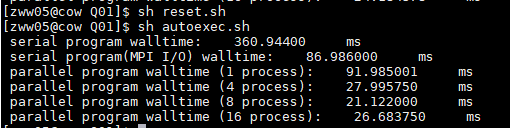
\includegraphics[width=0.9\linewidth]{Q01.png}
\end{center}

在程序执行的过程中,初始的串行程序和并行程序采用了不同的I/O方式,从而导致串行程序比1进程并行程序用时多出3倍的问题。通过将串行程序的I/O从Fortran自带的I/O更改为MPI的I/O之后,程序的计算结果符合估计。

从程序执行结果可以看出,当进程数为1时,并行程序慢于串行程序;随着进程数的增加,程序运行时间并没有越来越短,而是在减少到一定程度后反而随着进程数的增加而变长。产生该现象的原因是单个进程并行时计算量与串行相差不多,并行程序比串行程序多出了进程通信的开销;进程数过多时由于计算的规模并不是很大,通信开销的增长快于计算量的下降。可以估计,当矩阵$A$的维度增大时,采用16进程计算的并行程序用时会短于8进程的并行程序。

根据程序输出结果,计算并行度和效率并列成如下表格:

\begin{center}
	\begin{tabular}{c|c|c|c|c|c|c}
		\toprule
		\diagbox{运行结果}{进程数} & --(串行程序) & --(串行程序+MPI I/O) & 1 & 4 & 8 & 16\\
		\hline
		运行时间(ms) & 360.94 & 86.99 & 91.99 & 28.00 & 21.12 & 26.68\\
		\hline
		加速比 & -- & -- & 0.95 & 3.11 & 4.12 & 3.26\\
		\hline
		效率(\%) & -- & -- & 94.56 & 77.67 & 51.24 & 20.69\\
		\bottomrule
	\end{tabular}
\end{center}

从表格中的结果也可以看出,随着进程数的增加,并行效率越来越低,主要是由于通信开销增大导致。由于机器的限制,并未能成功测试$10240\times 10240$的矩阵向量乘法,可以推测计算较大的矩阵向量相乘时效率和加速比都会提高。

%%%%%%%%%%%%%%%%%%%%%%%%%%%%%%%%%%%%%%%%%%%%%%%%%%%%%%%%%%%%%%%%%%%%%%%%%
%%%%%%%%%%%%%%%%%%%%%%%%%%%%%%%%%%%%%%%%%%%%%%%%%%%%%%%%%%%%%%%%%%%%%%%%%
\section{并行五点差分法}
\subsection{问题描述与算法编程实现}
已知Possion方程
	
\begin{equation}
	\left\{
	\begin{aligned}
	\frac{\partial^{2}u}{\partial x^{2}}+\frac{\partial^{2}u}{\partial y^{2}}=xy,\quad (x,y)\in (0,1)\times (0,1)\\
	u(0,y)=y,u(1,y)=1-y,u(x,0)=0,u(x,1)=0
	\end{aligned}
	\right.
\end{equation}

采用五点差分法将方程离散为线性方程组,其中步长为$\frac{1}{50}$,写成矩阵运算的形式;采用红黑迭代法并行求解,给出并行算法的流程图,在并行机上编程实现,且针对处理机台数为$1,2,4,6,8$的情况下,给出并行率,讨论算法的可扩发性;提出改进的方法。

五点差分法在求解区域的网格节点上用其相邻四个节点上解的差商近似代替偏导数的离散方法,对于给定的Possion方程,五点差分格式为

$$\frac{u_{i,j+1}-2u_{i,j}+u_{i,j-1}}{h^{2}}+\frac{u_{i+1,j}-2u_{i,j}+u_{i-1,j}}{h^{2}}=h^{2}ij$$

其中$h=1/N=1/50$。将其写为矩阵运算$Au=F$,$u$表示各个节点的近似解。计算时需要将待求解的二维节点区域用一个向量表示,参考C语言中二维数组的表示方法,用向量$u$的$i+j\times (N+1)$个元素表示节点$(i,j)$处的近似解。根据五点差分的格式,$(i,j)$对应的$A$中的系数为$-4$,$(i+1,j),(i-1,j),(i,j+1),(i,j-1)$对应的系数为$1$,$A$是一个$(N+1)^{2}\times(N+1)^{2}$的矩阵。据此可以编写如下生成系数矩阵$A$和右端项$F$的程序。

\begin{center}
	\setlength{\fboxsep}{0.3pt}
	\lstset{
		language={[90]Fortran},
		extendedchars=false,
		lineskip=-1pt,
		basicstyle=\ttfamily\footnotesize\color{black},
		keywordstyle=\bf,
		showstringspaces=true,
		numberstyle=\color{black},
		%texcl=false,
		escapeinside=``,
		numbers=left,
		frame=single
	}
	\lstinputlisting{fdm_generate_matrix.f90}
	%\lstinputlisting{matrix_mul_vector_serial.f90}
	%\lstinputlisting{matrix_mul_vector_serial_with_mpi.f90}
\end{center}

其中$\textrm{MODULE constant\_}$中申明了程序中的常量。

\begin{center}
	\setlength{\fboxsep}{0.3pt}
	\lstset{
		language={[90]Fortran},
		extendedchars=false,
		lineskip=-1pt,
		basicstyle=\ttfamily\footnotesize\color{black},
		keywordstyle=\bf,
		showstringspaces=true,
		numberstyle=\color{black},
		%texcl=false,
		escapeinside=``,
		numbers=left,
		frame=single
	}
	\lstinputlisting{fdm_constant.f90}
\end{center}

生成系数矩阵后,将给出的边界条件整合到系数矩阵中。经过实际计算发现,如果不对矩阵的边界条件进行处理,得到的矩阵无法进行红黑排序,因此需要通过行变换将边界非对角元消去,同时对右端项进行相同的处理。这样处理之后的矩阵在去掉边界部分后可以通过红黑排序变换为一个$2\times 2$分块矩阵,其两个对角块均是对角矩阵。处理边界条件的程序如下。

\begin{center}
	\setlength{\fboxsep}{0.3pt}
	\lstset{
		language={[90]Fortran},
		extendedchars=false,
		lineskip=-1pt,
		basicstyle=\ttfamily\footnotesize\color{black},
		keywordstyle=\bf,
		showstringspaces=true,
		numberstyle=\color{black},
		%texcl=false,
		escapeinside=``,
		numbers=left,
		frame=single
	}
	\lstinputlisting{fdm_boundray_condition.f90}
\end{center}

在编写程序时,处理完边界条件后的矩阵依旧赋值给了原矩阵,但是处理完边界条件后的矩阵和原矩阵维度并不相同,在后续调用的时候需要注意调用该函数后系数矩阵和右端项矩阵只有一部分可以作为后续红黑排序的传入参数。更好的写法是返回一个制定大小的数组指针,避免产生该问题。

处理完边界条件后,为了并行化SOR迭代,需要对矩阵进行红黑排序。红黑排序以及多色排序的基本思想是利用排序技术,使排序后的矩阵可以分块为对角块是对角矩阵的形式,对网格点进行分类,使得任何一类网格点上值的更新只依赖于其他类网格点的值,同一类网格点之间的最新迭代值之间互不依赖。分组过程可以具体描述如下:用$l$记录所采用颜色的种数,$I$记录所有节点组成的集合,$c$记录各个节点所分配的颜色号,$T$记录已标记过颜色的节点集合,$S$记录尚未标颜色的节点集合,$\textrm{adj}_{k}$表示节点$k$的邻节点所组成的集合,辅助数组$t$用$t_{i}=0$或$1$表示颜色$i$在邻节点中没有/已经被使用过。多色排序的算法由如下的伪代码给出。

\begin{CJK*}{UTF8}{gkai}
	\begin{algorithm}
		\caption{多色排序}
		\begin{algorithmic}[1] %每行显示行号
			\State $l \gets 0,c_{1}\gets l,I \gets \{1,2,\cdots,n\},T\gets \{1\}$
			\For{$i = 2\to n$} $c_{i}\gets 0$
			\EndFor
			\For{$i = 1\to n$} $t_{i}\gets 0$
			\EndFor
			\While{$T \neq \{1,2,\cdots,n\}$}
				\State $S\gets I\ T,\textrm{Select} k\in S$
				\For{$j\in \textrm{adj}_{k}\cap T$}  $t_{c_{j}}\gets 1$
				\EndFor
				\For{$j = 1\to n$}
					\If{$t_{j} = 0$} $\textrm{Break}$ 
					\EndIf
				\EndFor
				\State $c_{j}\gets j$
				\If{$j = l+1$} $l\gets l+1$
				\EndIf
				\For{$j\in \textrm{adj}_{k}\cap T$} $t_{c_{j}}\gets 0$
				\EndFor
				\State $T \gets T\cup \{k\}$
			\EndWhile
		\end{algorithmic}
	\end{algorithm}
\end{CJK*}

在对矩阵多色排序之后,矩阵变为如下形式:

$$\left[\begin{matrix}
D_{R} & C_{1}\\
C_{2} & D_{B}
\end{matrix}\right]$$

其中$D_{R},D_{B}$是对角矩阵。对右端项做相同的分类,则方程$Au=F$可以写成

$$\left[\begin{matrix}
D_{R} & C_{1}\\
C_{2} & D_{B}
\end{matrix}\right]
\left[\begin{matrix}
U_{R}\\
U_{B}
\end{matrix}\right]=
\left[\begin{matrix}
F_{R}\\
F_{B}
\end{matrix}\right]$$

对应的SOR迭代格式为

$$\left[\begin{matrix}
D_{R} & \\
\omega C_{2} & D_{B}
\end{matrix}\right]
\left[\begin{matrix}
U_{R}^{k+1}\\
U_{B}^{k+1}
\end{matrix}\right]=
\left[\begin{matrix}
(1-\omega)D_{R} & -\omega C_{1}\\
& (1-\omega)D_{B}
\end{matrix}\right]
\left[\begin{matrix}
U_{R}^{k}\\
U_{B}^{k}
\end{matrix}\right]+
\omega
\left[\begin{matrix}
F_{R}\\
F_{B}
\end{matrix}\right]$$

与SOR迭代$(D-\omega L)U^{k+1}=(\omega U+(1-\omega)D)U^{k}+\omega F$相比可以看出,红黑排序后在每组节点的计算中,不依赖于同类节点最新的迭代值,具有较好的并行性。红黑排序的程序如下。

\begin{center}
	\setlength{\fboxsep}{0.3pt}
	\lstset{
		language={[90]Fortran},
		extendedchars=false,
		lineskip=-1pt,
		basicstyle=\ttfamily\footnotesize\color{black},
		keywordstyle=\bf,
		showstringspaces=true,
		numberstyle=\color{black},
		%texcl=false,
		escapeinside=``,
		numbers=left,
		frame=single
	}
	\lstinputlisting{fdm_sortRB.f90}
\end{center}

将以上子程序组装为一个完整的程序,并将排序后的矩阵输出到文件中用于后续计算。同时,为了编写串行的SOR程序,将排序前的矩阵也输出到文件中。

\begin{center}
	\setlength{\fboxsep}{0.3pt}
	\lstset{
		language={[90]Fortran},
		extendedchars=false,
		lineskip=-1pt,
		basicstyle=\ttfamily\footnotesize\color{black},
		keywordstyle=\bf,
		showstringspaces=true,
		numberstyle=\color{black},
		%texcl=false,
		escapeinside=``,
		numbers=left,
		frame=single
	}
	\lstinputlisting{fdm_matrix.f90}
\end{center}


%%%%%%%%%%%%%%%%%%%%%%%%%%%%%%%%%%%%%%%%%%%%%%%%%%%%%%%%%%%%%%%%%%%%%%%%%
\subsection{运行结果与分析}


\end{document}